\documentclass{article}
\usepackage{tikz}
\usetikzlibrary{trees}

\begin{document}

\begin{figure}[h]
    \centering
    \begin{tikzpicture}[
        level 1/.style={sibling distance=30mm},
        level 2/.style={sibling distance=10mm},
        edge from parent/.style={draw,-latex}
    ]
        \node {4}
            child {node {4}}
            child {node {1}}
            child {node {1}}
            child {node {1}};
    \end{tikzpicture}
    \caption{$|Simp_{4}| \cdot |Simp_{4}| \cdot 4 = 16$}
    
    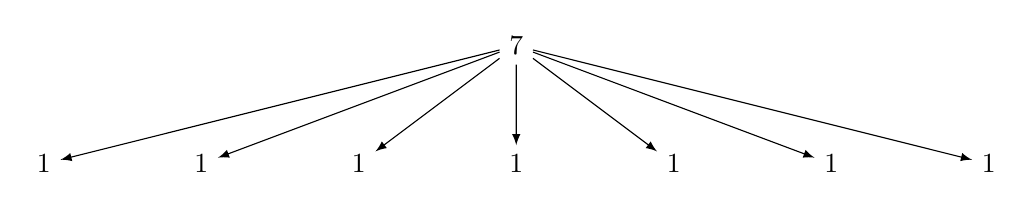
\begin{tikzpicture}[
        level 1/.style={sibling distance=20mm},
        level 2/.style={sibling distance=10mm},
        level 3/.style={sibling distance=10mm},
        edge from parent/.style={draw,-latex}
    ]
        \node {7}
            child {node {1}}
            child {node {1}}
            child {node {1}}
            child {node {1}}
            child {node {1}}
            child {node {1}}
            child {node {1}};
    \end{tikzpicture}
    \caption{$|Simp_{7}| = 338$}
\end{figure}

\end{document}